\documentclass[tikz]{standalone}
\usepackage{amsmath}
\usetikzlibrary{calc,backgrounds}
\definecolor{bgcol}{HTML}{171D2B}
\definecolor{accent}{HTML}{F7B538}
\definecolor{linecol}{HTML}{8FA3BF}
\begin{document}
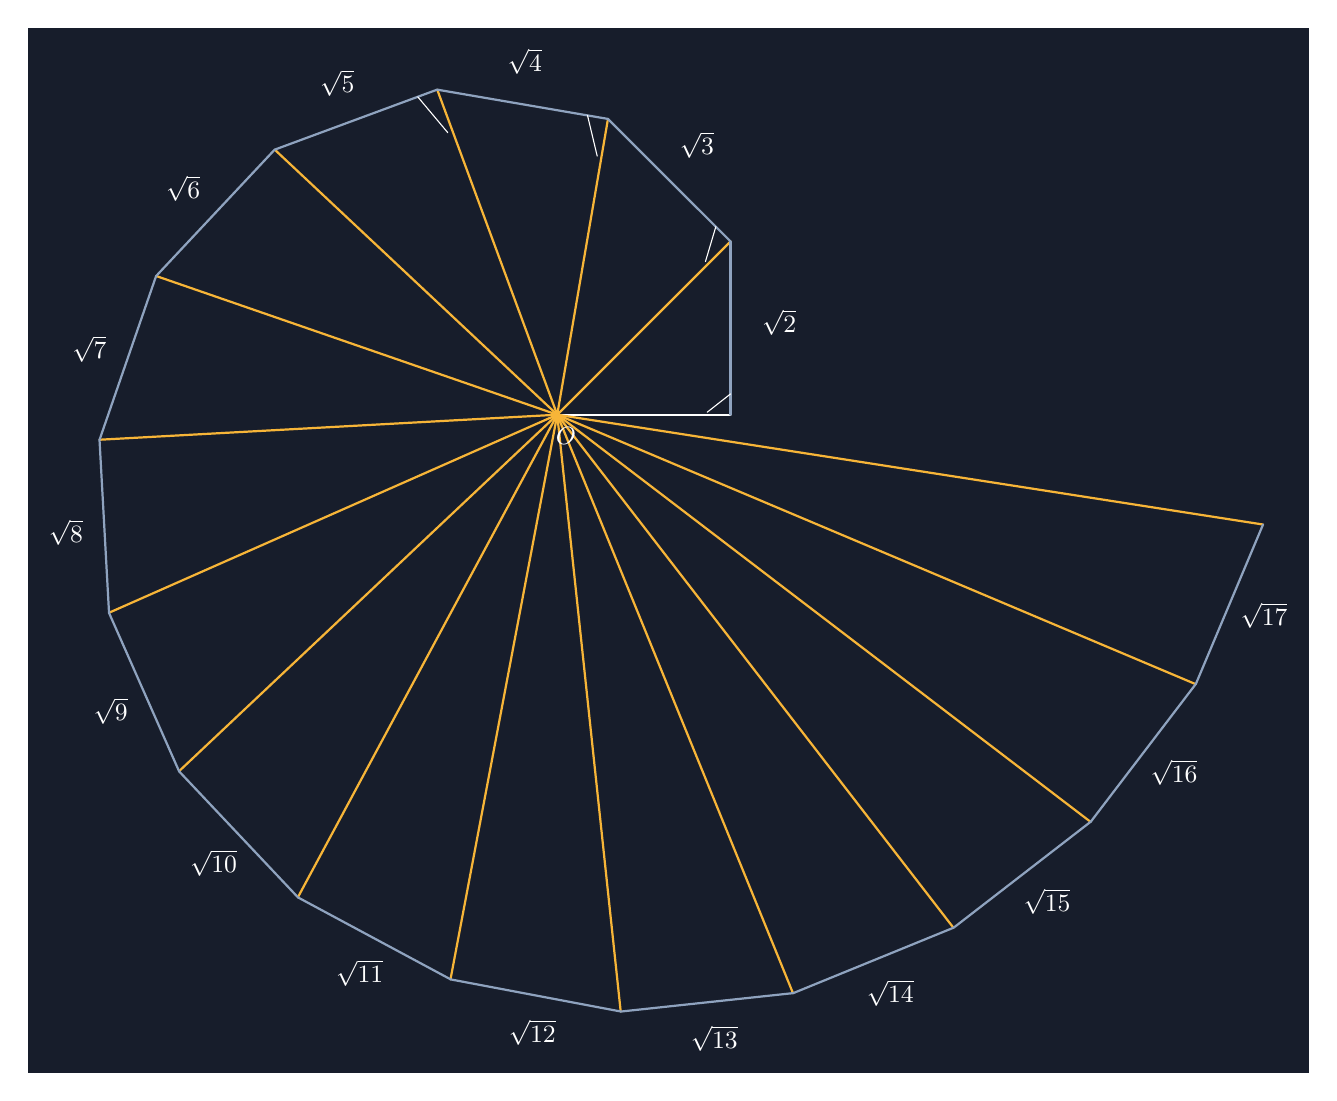
\begin{tikzpicture}[background rectangle/.style={fill=bgcol}, show background rectangle,
  scale=2.2, line cap=round]
  \pgfmathsetmacro{\angleAcc}{0}
  \coordinate (O) at (0,0);
  \coordinate (P) at (1,0);
  \draw[white, thick] (O) -- (P);
  \foreach \n in {1,...,16}{
    \pgfmathsetmacro{\step}{atan2(1, sqrt(\n))}
    \pgfmathsetmacro{\angleAcc}{\angleAcc + \step}
    \pgfmathsetmacro{\r}{sqrt(\n+1)}
    \coordinate (Q) at ({\r*cos(\angleAcc)},{\r*sin(\angleAcc)});
    \draw[accent, thick] (O) -- (Q);
    \draw[linecol, thick] (P) -- (Q);
    \pgfmathsetmacro{\midang}{\angleAcc - \step/2}
    \pgfmathsetmacro{\midr}{(\r + sqrt(\n))/2 + 0.18}
    \node[white, font=\small] at ({\midang}:{\midr}) {$\sqrt{\the\numexpr\n+1\relax}$};
    \ifnum\n<5
      \coordinate (A) at ($(P)!0.12!(O)$);
      \coordinate (B) at ($(P)!0.12!(Q)$);
      \draw[white] ($(A)!0.12!90:(B)$) -- (B);
    \fi
    \global\let\angleAcc\angleAcc
    \coordinate (P) at (Q);
  }
  \node[white, font=\small] at (0.05,-0.12) {$O$};
\end{tikzpicture}
\end{document}
